\documentclass[10pt,a4paper]{report}
\usepackage[latin1]{inputenc}
\usepackage{amsmath}
\usepackage{amsfonts}
\usepackage{amssymb}
\usepackage{graphicx}
\author{William Seymour}
\title{Dissertation Progress Review}
\date{\today}
\begin{document}
\maketitle

\section*{Introduction}
The project aims to explore how gamification and analytics can be used in the design of educational software. Gamification is a fairly young field of study, the term having only really gained popularity in late 2010 as shown in figure \ref{usage} (Google 2014).

In addition to the study of gamification, the project also seeks to provide an example of how analytics can be used to support lecturers and allow them to better use their time when teaching in a higher education context. This will be achieved by suggesting topics and delivery methods for guided one to one or seminar style tuition in an attempt to reinforce the progress made by students online. It will also be possible to match students who share learning styles and strength/weakness pairings in specific subject areas.

Construction of a web platform capable of the aforementioned functionality is a daunting undertaking, and the research required for it to be effective in it's aims will be substantial. Taking on a project in an exciting and relatively new field is proving to be both stimulating and rewarding.
\begin{figure}
	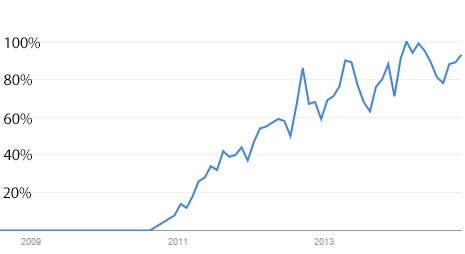
\includegraphics{../img/usage-graph.png}
	\caption{Usage of the term 'gamification' as a proportion of google searches, from 2009 to the present day (Google 2014)}
	\label{usage}
\end{figure}
\section*{Background Research}
\section*{Technical content}
\section*{Progress}
\section*{Next Steps}
\section*{Appraisal}
\section*{Ethics}
\section*{Project Management}
\section*{Conclusion}
\section*{Table of Figures}
\listoffigures
\section*{Appendices}
\section*{Bibliography}
Google, 2014. \textit{Google Trends- Web Search interest: gamification - Worldwide, 2009 - 2014}. [image online] Available at: $\langle$http://www.google.com/trends/explore\#q=gamification\&date=1\%2F2009\%2072m\&cmpt=q$\rangle$ [Accessed 09/11/2014].
\end{document}